% !TEX root = ../main.tex
\paragraph{Low Threshold Cherenkov Counter (LTCC)}
    \begin{wrapfigure}{l}{0.50\textwidth}
        \centering\frame{
        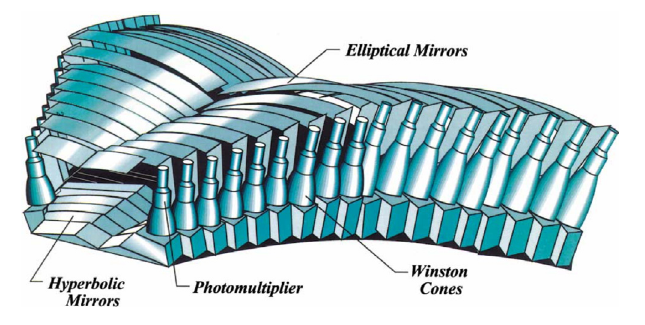
\includegraphics[width=\linewidth]{213ltcc.png}}
        \caption[LTCC Mirror System]{Layout and components of the optical mirror system within each LTCC box from the design model.
        Source: \hyperlink{jlab.org/physics/hall-b/clas12}{CLAS12 wiki}.}
        \label{fig::11.213::ltcc}
    \end{wrapfigure}

    The LTCC system in CLAS12 is designed for the detection of charged pions and kaons in the momentum range of $3.5$ to $9 ~\text{GeV}$.
    It consists of boxes shaped like truncated pyramids, with four out of the six sectors of CLAS12 equipped with one LTCC box.
    Each LTCC box contains 108 lightweight mirrors with composite backing structures, 36 Winston light-collecting cones, 36 125-mm diameter PMTs, and 36 magnetic shields.
    The LTCC boxes are filled with heavy C4 F10 radiator gas.

    As part of the 12 GeV upgrade, the LTCC detector from the previous CLAS experiment was refurbished to enhance its efficiency for charged pion and kaon detection.
    The enhancements included increasing the volume of the radiator gas, refurbishing the elliptical and hyperbolic mirrors with new coatings, and improving the sensitivity of the PMTs to Cherenkov light.
    The sensitivity improvement was achieved by coating the entrance windows of the PMTs with a wavelength-shifting material.
    This material absorbs ultraviolet (UV) light with wavelengths below $300 ~\text{nm}$ and re-emits two photons at a larger wavelength.
    These enhancements aim to improve the overall performance and detection efficiency of the LTCC system \cite{ungaro2020}.
    A drawing from the design model of the LTCC can be seen in Figure \ref{fig::11.213::ltcc}.
